%\documentclass[preprint,tightenlines,showpacs,showkeys,floatfix,
%nofootinbib,superscriptaddress,fleqn]{revtex4} 
\documentclass[tightenlines,floatfix,nofootinbib,superscriptaddress,fleqn]{revtex4} 
%\documentclass[aps,epsfig,tightlines,fleqn]{revtex4}
\usepackage{kotex}
\usepackage[HWP]{dhucs-interword}
\usepackage[dvips]{color}
\usepackage{graphicx}
\usepackage{bm}
%\usepackage{fancyhdr}
%\usepackage{dcolumn}
\usepackage{defcolor}
\usepackage{amsmath}
\usepackage{amsfonts}
\usepackage{amssymb}
\usepackage{amscd}
\usepackage{amsthm}
\usepackage[utf8]{inputenc}
%\pagestyle{fancy}

\begin{document}

\title{\Large 2022년 2학기 물리학 II}
\author{김현철\footnote{Office: 5S-436D (면담시간 매주
    수요일-16:15$\sim$18:00)}} 
\email{hchkim@inha.ac.kr}
\affiliation{Hadron Theory Group, Department of Physics,
  Inha  University, Incheon 22212, Republic of Korea }
\date{Autumn Semester, 2020}

\maketitle

{\color{red} {\bf Due date:} 2022년 9월 7일  15:30-16:15 }
\vspace{1.cm}

\noindent \textbf{ 주의: \color{blue} 단 한 번의 부정행위도 절대
  용납하지 않습니다. 적발 시, 학점은 F를 받게 됨은 물론이고,
  징계위원회에 회부합니다. One strike out임을 명심하세요.} 
\\
\\

{\bf 학번:} \hspace{4cm}
{\bf 이름:} 

\section*{\large Quiz 4}
\noindent {\bf 문제 1 [10pt].} 다음의 질문에 답하세요.
\begin{itemize}
\item[(가)] 점전하에서부터 $r$ 만큼 떨어진 곳에서 전기퍼텐셜을
  구하세요.
\item[(나)] $d$만큼 떨어져서 서로 나란히 마주보고 있는 무한 평면판이
  있다. 왼쪽 판에는 면전하밀도 $+\sigma$로 대전되어 있고, 오른쪽
  판에는 $-\sigma$로 대전되어 있을 때 두 평면판 사이의 전위차를
  구하여라. 
\item[(다)] 반지름이 $r$인 구형 도체 표면에서 전기퍼텐셜이 $V_0$로
  주어졌을 때 그 도체의 중심에서 전기퍼텐셜은 얼마인가? 
\end{itemize}
\newpage
{\color{gray} [문제 풀이 쪽]}
\newpage

\noindent {\bf 문제 2 [10pt].} 
그림~\ref{fig:1}처럼 두 전하가 거리
$d=2.00$ cm만큼 떨어져서 놓여있다. 여기서 $Q=+5.00$ nC이다. 
\begin{figure}[htp]
  \centering
  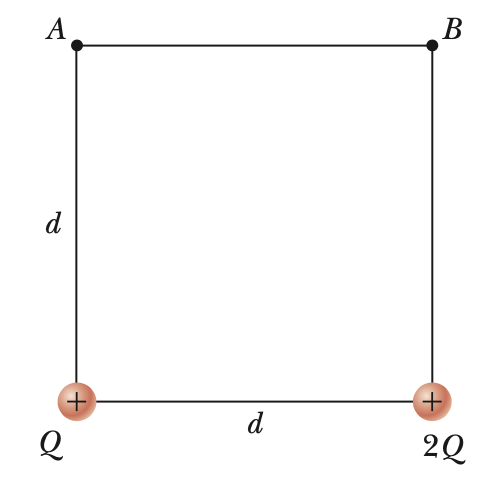
\includegraphics[scale=0.6]{qfig5-1.png}
  \caption{\textbf{문제 2}}
  \label{fig:1}
\end{figure}
\begin{itemize}
\item[(가)] $A$에서 전위를 구하여라.
\item[(나)] $B$에서 전위를 구하여라.
\item[(다)] $A$와 $B$ 사이의 전위차를 구하여라.
\end{itemize}
\newpage
{\color{gray} [문제 풀이 쪽]}
\newpage

\noindent {\bf 문제 3 [20pt].} 
그림~\ref{fig:2}에서처럼 바깥쪽 반지름이
$R=13$ cm이고, 안쪽 반지름이 $r=0.2R$인 고리가 있다.
\begin{figure}[htp]
  \centering
  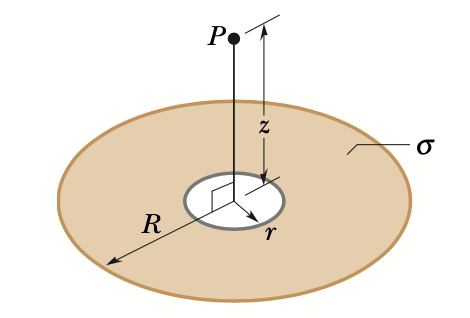
\includegraphics[scale=0.6]{qfig5-2.png}
  \caption{\textbf{문제 3}}
  \label{fig:2}
\end{figure}
 면전하 밀도는
$\sigma=6.20\,\mathrm{pC/m^2}$으로 균일하다. 무한대에서 $V=0$일 때,
고리의 중앙으로부터 거리 $z=2R$만큼 떨어진 점 $P$에서 전위를 구하여라. 
\newpage
{\color{gray} [문제 풀이 쪽]}
\newpage

\noindent {\bf 문제 4 [50pt].} 
전하량이 $30.0$ pC($1\,\mathrm{pC} = 10^{-12}\,\mathrm{pC}$)인 어떤
물방울의 표면에서 전위는 $500$ V이다. 
\begin{itemize}
\item[(가)] 이 물방울의 반지름은 얼마인가?  
\item[(나)] 이런 물방울 두 개가 서로 뭉치면 표면 전위는 얼마인가? 
\end{itemize}
\newpage
{\color{gray} [문제 풀이 쪽]}

\end{document}